\section{Preliminaries}
\label{section:preliminaries}

In this section, we focus on the vocabulary used in this report, along with the first known results required for the next sections. Let us start with some notation that will be used throughout this report. For an integer $k$, by $[k]$ we denote $\{1, \dots, k\}$. For a graph $G$, by $V(G)$ we denote the set of vertices of $G$ and by $E(G)$ we denote the set of edges of $G$. If $X \subseteq V(G)$, then $G - X$ denotes the graph obtained by removing every vertex in $X$ and every edge with an endpoint in $X$. Unless stated otherwise, $n$ always refers to $|V(G)|$, while $m$ refers to $|E(G)|$. 
% For a set $X$, by $X = X_1 \uplus \dots \uplus X_m$ we denote a disjoint partition of $X$.
%  (i.e. $X_1 \cup \dots \cup X_m = X$ and $X_i \cap X_j = \emptyset$ for every $1 \leq i < j \leq m$).

\medskip

In this report, the four following \NP-hard problems will be discussed:

\begin{problem}
    \problemtitle{VertexCover}
    \probleminput{A graph $G = (V, E)$, an integer $k$}
    \problemquestion{Does there exist a subset of vertices $X\subseteq V$ such that $|X| \leq k$ and every edge in $E$ has at least one endpoint in $X$?}
\end{problem}

\begin{problem}
    \problemtitle{IndependentSet}
    \probleminput{A graph $G = (V, E)$, an integer $k$}
    \problemquestion{Does there exist a subset of vertices $X \subseteq V$ such that $|X| \geq k$ and no vertices in $X$ are adjacent?}
\end{problem}

\begin{problem}
    \problemtitle{$q$-Coloring}
    \probleminput{A graph $G = (V, E)$}
    \problemquestion{Can the vertices of $G$ be colored with $q$ colors such that no two adjacent vertices share the same color. In other words, does there exist a function $f : V \mapsto [q]$ where $f(u) \neq f(v)$ for every edge $\{u,v\} \in E$?}
\end{problem}

% \begin{problem}
%     \problemtitle{MaxCut}
%     \probleminput{A graph $G = (V, E)$, an integer $k$}
%     \problemquestion{Can the vertex set $V$ be partitioned into two disjoint subsets, $V = V_1 \uplus V_2$, such that the number of edges between $V_1$ and $V_2$ is at least $k$?}
% \end{problem}

% \begin{problem}
%     \problemtitle{OddCycleTransversal}
%     \probleminput{A graph $G = (V, E)$, an integer $k$}
%     \problemquestion{Does there exist a subset of vertices $X \subseteq V$ such that $|X| \leq k$ and $G - X$ is bipartite?}
% \end{problem}

\begin{problem}
    \problemtitle{DominatingSet}
    \probleminput{A graph $G = (V, E)$, an integer $k$}
    \problemquestion{Does there exist a subset of vertices $D \subseteq V$ such that $|D| \leq k$ and every vertex in $V$ is either in $D$ or adjacent to a vertex in $D$?}
\end{problem}

\subsection{Parameters}

In this section, we define the various graph parameters used throughout this report.

\subsubsection*{Treewidth}

In \refsec{section:introduction}, we gave an informal description of the treewidth of a graph $G$ as a measure of its "tree-like" structure. Let us now formally define it. This parameter can be defined using the concept of a \textit{tree decomposition}, concept initially introduced by Robertson and Seymour in their seminal work on graph minors \cite{robertson1986graph}.

\begin{definition}[tree decomposition]
    A tree decomposition of a graph $G$ is a pair $(T, \{X_i\}_{i \in V(T)})$ where $T$ is a tree and $\{X_i\}_{i \in V(T)}$ is a collection of subsets of $V(G)$ (called \emph{bags}) such that:
    \begin{enumerate}
        \item For every vertex $v \in V(G)$, there exists at least one bag $X_i$ such that $v \in X_i$.
        \item For every edge $\{u, v\} \in E(G)$ , there exists at least one bag $X_i$ such that $\{u, v\} \subseteq X_i$.
        \item For every vertex $v \in V$, the set $\{i\ |\ v \in X_i\}$ forms a connected subtree of $T$.
    \end{enumerate}
\end{definition}

\begin{definition}[width of a tree decomposition]
    The width of a tree decomposition $(T,\{X_i\}_{i \in V(T)})$ is the size of the biggest bag of the decomposition minus 1. Formally, it is defined as $\max_{i \in V(T)} |X_i| - 1$.
\end{definition}

\begin{definition}[treewidth]
    The treewidth of a graph $G$ is the smallest integer $k$ such that $G$ has a tree decomposition where each bag contains at most $k+1$ vertices.
\end{definition}

Although the formal definition may not immediately convey the intuition behind this measure, we provide examples in \reffigure{fig:treewidth-example} to illustrate how treewidth captures the tree-like structure of a graph.

\begin{figure}
    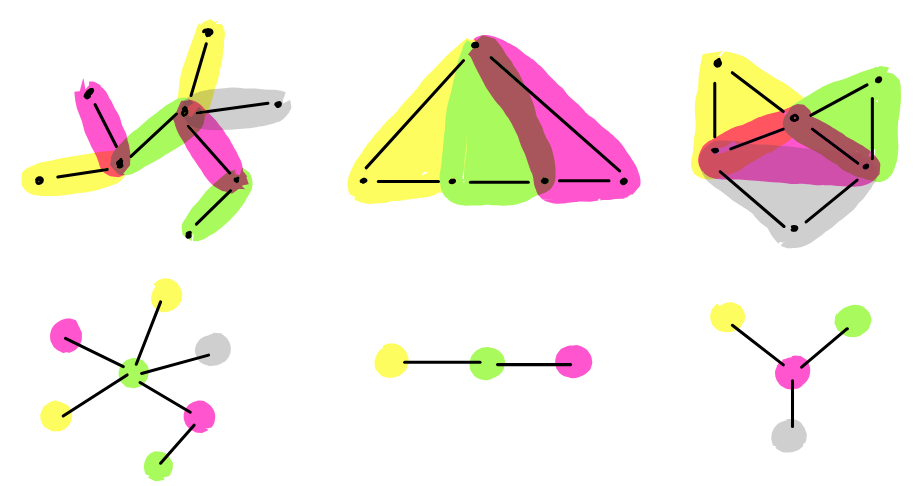
\includegraphics[width=\textwidth]{figures/treewidth-example.png}
    \caption{Examples of treewidth. (a) A tree has treewidth 1. (b) A cycle has treewidth 2. (c) A graph with treewidth 2. For each example, the bags of a tree decomposition of the graph is shown at the top, and the tree of the corresponding tree decomposition is depicted at the bottom.}
    \label{fig:treewidth-example}
\end{figure} 

\subsubsection*{Pathwidth}

Alongside treewidth, we can also consider the \textit{pathwidth} of a graph $G$, denoted $\pw(G)$. This parameter has the same definition as treewidth, except that a tree decomposition is replaced by a \textit{path decomposition} which is a pair $(P, \{X_i\}_{i \in V(P)})$ where $P$ is a path.

\subsubsection*{Treedepth}

Another parameter that is somewhat similar to treewidth is the \textit{treedepth} of a graph $G$. Various definitions exist in the literature for this parameter, and we adopt the definition provided by Ne{\v{s}}et{\v{r}}il and Ossona de Mendez \cite{nevsetvril2006tree}, which employs the concept of an \textit{elimination forest}.

\begin{definition}[elimination forest]
    An elimination forest of a graph $G$ is a pair $(F, f)$ where $F$ is a rooted forest and $f : V(G) \mapsto V(F)$ is a bijection that maps vertices of $G$ to vertices of the forest $F$. This mapping satisfies the property that if $\{u, v\} \in E(G)$ then either $f(u)$ is an ancestor of $f(v)$, or $f(v)$ is an ancestor of $f(u)$.
\end{definition}

\begin{definition}[depth of an elimination forest]
    The depth of an elimination forest $(F, f)$ is defined as the depth of $F$, which is the length of the longest path between one root and a leaf in a tree of $F$.
\end{definition}

\begin{definition}[treedepth]
    The treedepth of a graph $G$, denoted $\td(G)$, is defined as the minimum depth over all possible elimination forests of $G$. Formally, $\td(G) = \min_{(F, f)} d(F)$, where $d(F)$ denotes the depth of the rooted forest $F$.
\end{definition}

Some examples of elimination forests are shown in \reffigure{fig:treedepth-example}.

\begin{figure}
    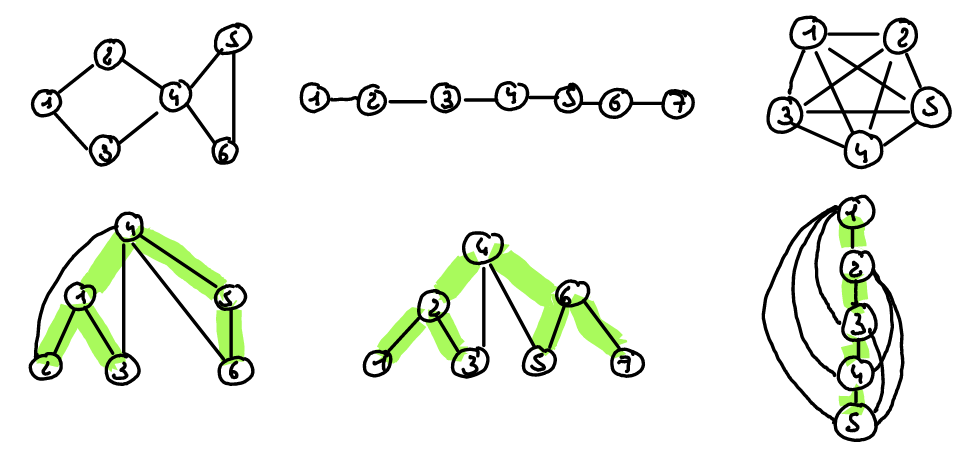
\includegraphics[width=\textwidth]{figures/treedepth-example.png}
    \caption{Examples of treedepth. (a) A graph with treedepth 3. (b) A path of size $n$ has treedepth $\lceil\log_2(n)\rceil$. (c) A clique of size $n$ has treedepth $n$. For each example, the graph is shown at the top, and the elimination forest is depicted in green at the bottom.}
    \label{fig:treedepth-example}
\end{figure}

\subsubsection*{$\F$-modulator}

Let $\F$ be a class of graphs and $G$ be a graph. We say that $X \subseteq V(G)$ is an \emph{$\F$-modulator} of $G$ if $G - X \in \F$. The size of an $\F$-modulator can be used as a parameter. In this report, we will use some of these parameters for different choices of $\F$, most of them have their own specific names:

\begin{itemize}
    \item Let $\F$ be \graphclass{IndependentSet}, the class of all graphs without edges. Then an $\F$-modulator is a \textit{vertex cover}, and the corresponding parameter is denoted by $\vc$.
    \item Let $\F$ be \graphclass{Bipartite}, the class of all graphs without odd cycles. Then an $\F$-modulator is an \textit{odd cycle transversal}, and the corresponding parameter is denoted by $\oct$.
    \item Let $\F$ be \graphclass{Forest}, the class of all graphs without cycles. Then an $\F$-modulator is a \textit{feedback vertex set}, and the corresponding parameter is denoted by $\fvs$.
    \item Let $\F$ be \graphclass{LinearForest}, the class of all graphs without cycles and where the maximum degree of a vertex is 2. Then an $\F$-modulator is a \textit{linear feedback vertex set}, and the corresponding parameter is denoted by $\lfvs$.
    \item Let $\F$ be \graphclass{$\sigma$-ConnectedComponent}, the class of all graphs without connected components of size more than $\sigma$. Then an $\F$-modulator is a \textit{$\sigma$-hub}, and the corresponding parameter is denoted by $\shub$.
\end{itemize}

\medskip

We will consider an additional case for $\sigma$-hub: when the number of edges between each component and a $\sigma$-hub is bounded by a constant $\delta$, we say that the hub is a \textit{$(\sigma, \delta)$-hub}, and the parameter is denoted $\sdhub$ \cite{esmer2024fundamental}.

Examples illustrating each of these parameters can be seen in \reffigure{fig:fkv-graph-example}.

\begin{figure}
    \centering
    \begin{subfigure}[b]{0.22\textwidth}
        \adjincludegraphics[width=\textwidth,trim={0 0 {.78\width} 0},clip]{figures/fkv-graph-example.png}
        \caption{A vertex cover of size 7.}
    \end{subfigure}
    \hspace{1cm}
    \begin{subfigure}[b]{0.22\textwidth}
        \adjincludegraphics[width=\textwidth,trim={{.22\width} 0 {.56\width} 0},clip]{figures/fkv-graph-example.png}
        \caption{A feedback vertex set of size 6.}
    \end{subfigure}
    \hspace{1cm}
    \begin{subfigure}[b]{0.18\textwidth}
        \adjincludegraphics[width=\textwidth,trim={{.44\width} 0 {.38\width} 0},clip]{figures/fkv-graph-example.png}
        \caption{A linear feedback vertex set of size 5.}
    \end{subfigure}

    \begin{subfigure}[b]{0.18\textwidth}
        \adjincludegraphics[width=\textwidth,trim={{.62\width} 0 {.2\width} 0},clip]{figures/fkv-graph-example.png}
        \caption{An odd cycle transversal of size 8.}
    \end{subfigure}
    \hspace{1cm}
    \begin{subfigure}[b]{0.2\textwidth}
        \adjincludegraphics[width=\textwidth,trim={{.8\width} 0 0 0},clip]{figures/fkv-graph-example.png}
        \caption{A $(4, 3)$-hub of size 9.}
    \end{subfigure}

    

    \caption{Examples of $\F$-modulators, with the $\F$-modulator drawn in red.}
    \label{fig:fkv-graph-example}
\end{figure}

\subsection{A hierarchy of parameters}

Some parameters are "stronger" than others in the sense that developing an algorithm based on them is more challenging because they provide more detailed information about the graph. For instance, finding an algorithm parameterized by pathwidth is generally easier than one parameterized by treewidth, since a path decomposition is a special case of a tree decomposition. Identifying correlations between these parameters is crucial, as it refines our understanding of which problems can be efficiently solved under specific parameters. This is why establishing a hierarchy of parameters is so important.

To establish a hierarchy of parameters, we first define how parameters can be compared. Formally, a parameter is a function $\pi$ that takes a graph as input and returns a number. For a pair of parameters $\pi_1, \pi_2$, we write $\pi_1 \lp \pi_2$ if there exists a constant $c$ such that for every graph $G$, $\pi_1(G) \leq \pi_2(G) + c$.

This subsection describes how the parameters defined above compare to each other. The final hierarchy is illustrated in \reffigure{fig:hierarchy}. A portion of this hierarchy is derived from \cite{fellows2013towards}. We encourage interested readers to consult this paper for further exploration of additional parameters and their relationships.

\begin{tikzpicture}
    \tikzstyle{vertex} = [draw=black,fill=black,circle,inner sep=0pt,minimum size=3pt];
    \tikzstyle{possible} = [fill=green,circle,inner sep=0pt,minimum size=10pt];
    \tikzstyle{impossible} = [fill=red,circle,inner sep=0pt,minimum size=10pt];
    \tikzstyle{new} = [fill=lime,circle,inner sep=0pt,minimum size=10pt];
    \tikzstyle{result} = [draw=black,circle,dashed,thick,inner sep=0pt,minimum size=20pt];
    \tikzstyle{edge} = [draw=black,thick];
    \tikzstyle{possibleedge} = [draw=green,line width=5pt];
    \tikzstyle{impossibleedge} = [draw=red,line width=5pt];
    \tikzstyle{newedge} = [draw=lime,line width=5pt];

    % This is an invisible rectangle which draw the picture to avoid nodes to move when appear/disappear.
    \path (0, 0) -- (3.2, 0) -- (3.2, 5) -- (0, 5);

    \coordinate (A) at (2, 4.6);
    \coordinate (B) at (2, 3.8);
    \coordinate (C) at (2, 3);
    \coordinate (D) at (1, 1.7);
    \coordinate (E) at (1, .7);
    \coordinate (F) at (0, 0);
    \coordinate (G) at (3.5, 3);
    \coordinate (H) at (3, 2.5);
    \coordinate (I) at (3, 1.5);
    \coordinate (J) at (3, .5);
    \coordinate (K) at (2, 0);

    \node<3-> [style=possible] at (A) {};
    \node<4-> [style=possible] at (B) {};
    \node<7-> [style=possible] at (G) {};

    \draw<4-> [style=possibleedge] (A) -- (B);

    \node<6-> [style=impossible] at (I) {};
    \node<5-> [style=impossible] at (J) {};
    \node<5-> [style=impossible] at (K) {};

    \draw<6-> [style=impossibleedge] (I) -- (J);
    \draw<5-> [style=impossibleedge] (J) -- (K);

    \node<8-> [style=new] at (C) {};
    \node<8-> [style=new] at (D) {};
    \node<8-> [style=new] at (E) {};
    \node<8-> [style=new] at (F) {};
    \node<9-> [style=new] at (H) {};

    \draw<8-> [style=newedge] (B) -- (C);
    \draw<8-> [style=newedge] (C) -- (D);
    \draw<9-> [style=newedge] (C) -- (H);
    \draw<8-> [style=newedge] (D) -- (E);
    \draw<8-> [style=newedge] (E) -- (F);
    \draw<9-> [style=newedge] (G) -- (H);

    \node<8-> [style=result] at (F) {};
    \node<9-> [style=result] at (H) {};
    \node<10-> [style=result] at (I) {};

    \node [style=vertex,label={[label distance=1pt]180:$n$}]        at (A) {};
    \node [style=vertex,label={[label distance=1pt]180:\vc}]        at (B) {};
    \node [style=vertex,label={[label distance=1pt]180:$\shub[2]$}] at (C) {};
    \node [style=vertex,label={[label distance=1pt]170:\lfvs}]      at (D) {};
    \node [style=vertex,label={[label distance=1pt]170:\fvs}]       at (E) {};
    \node [style=vertex,label={[label distance=1pt]270:\oct}]       at (F) {};
    \node [style=vertex,label={[label distance=1pt]90:$\sdhub$}]   at (G) {};
    \node [style=vertex,label={[label distance=1pt]0:$\shub$}]    at (H) {};
    \node [style=vertex,label={[label distance=1pt]0:\td}]        at (I) {};
    \node [style=vertex,label={[label distance=1pt]0:\pw}]        at (J) {};
    \node [style=vertex,label={[label distance=1pt]270:\tw}]        at (K) {};

    \draw [style=edge] (A) -- (B);
    \draw [style=edge] (B) -- (C);
    \draw [style=edge] (C) -- (D);
    \draw [style=edge] (C) -- (H);
    \draw [style=edge] (D) -- (E);
    \draw [style=edge] (D) -- (J);
    \draw [style=edge] (E) -- (F);
    \draw [style=edge] (E) -- (K);
    \draw [style=edge] (G) -- (H);
    \draw [style=edge] (H) -- (I);
    \draw [style=edge] (I) -- (J);
    \draw [style=edge] (J) -- (K);
\end{tikzpicture}

\subsubsection*{Treewidth $\lp$ pathwidth}

We can immediately see why $\tw \lp \pw$. Indeed, a path is a specific type of tree; thus, for any graph, a path decomposition is also a tree decomposition.

\subsubsection*{Pathwidth $\lp$ treedepth}

It is quite intuitive why $\pw \lp \td$. Indeed, given an elimination forest of a graph $G$, we can create a bag for every branch of the elimination forest. Then it can be verified that this forms a path decomposition of the graph, and we have $\pw(G) \leq \td(G)$. A pictorial intuition of this transformation is provided in \reffigure{fig:treedepth-to-pathwidth}.

\begin{figure}
    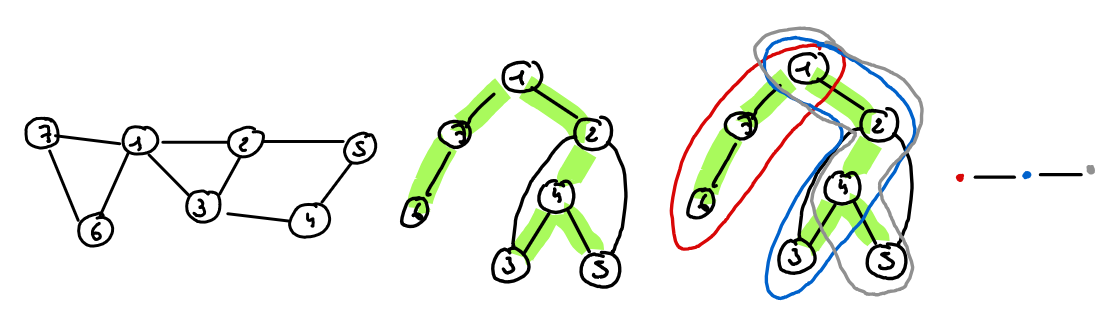
\includegraphics[width=\textwidth]{figures/treedepth-to-pathwidth.png}
    \caption{How to transform an elimination forest into a path decomposition. (a) A graph $G$. (b) An elimination forest of $G$. (c) Bags of a path decomposition of $G$ which follow the elimination forest. (d) The path decomposition of these bags. We can see that the depth of the elimination forest is the same as the width of the obtained path decomposition.}
    \label{fig:treedepth-to-pathwidth}
\end{figure}

\subsubsection*{Hierarchy of $\F$-modulators}

For $\F$-modulators, we have $\oct \lp \fvs \lp \lfvs \lp \shub[2] \lp \vc \lp n$. This is due to the fact that we have the following hierarchy of classes:
$$\graphclass{IndependentSet} \subseteq \graphclass{$2$-ConnectedComponent} \subseteq \graphclass{LinearForest} \subseteq \graphclass{Forest} \subseteq \graphclass{Bipartite}$$

The first inclusion is due to the fact that if $\sigma \leq \mu$, then $\sigma\graphclass{-ConnectedComponent} \subseteq \mu\graphclass{-ConnectedComponent}$. Moreover, \graphclass{IndependentSet} is the same class as \graphclass{$1$-ConnectedComponent}, since a graph without edges consists of disconnected components with only one vertex each and vice versa.

Now, if $\F_1 \subseteq \F_2$ and $X$ is an $\F_1$-modulator, then $X$ is also an $\F_2$-modulator. This explains why $\oct \lp \fvs \lp \lfvs \lp \shub[2] \lp \vc$. Following the same logic, a $\sdhub$ is also a $\shub$, which explains why $\shub \lp \sdhub$. Finally $\vc \lp n$ is simple: a vertex cover of a graph cannot have more vertices than the graph itself.

\subsubsection*{Treedepth $\lp \sdhub$}

Let $G$ be a graph with a $\shub$ $X$ of size $k$. The treedepth of $X$ is at most $k$ since we can arrange the vertices of $X$ in a linear fashion, forming a trivial elimination forest (see \reffigure{fig:shub-to-treedepth}). Removing $X$ leaves connected components of size at most $\sigma$, each having treedepth at most $\sigma$. Attaching the elimination forest of each component to the leaf of the elimination forest of $X$ results in a valid elimination forest for $G$ since the connected components have no common edges. This results in a total depth at most $k + \sigma$. Therefore, $\td(G) \leq \shub(G) + \sigma$, leading to $\td \lp \shub$ since $\sigma$ is a constant.

\begin{figure}
    \centering
    \begin{subfigure}[b]{0.33\textwidth}
        \adjincludegraphics[width=\textwidth,trim={0 0 {.45\width} 0},clip]{figures/shub-to-treedepth.png}
        \caption{}
    \end{subfigure}
    \begin{subfigure}[b]{0.27\textwidth}
        \adjincludegraphics[width=\textwidth,trim={{.55\width} 0 0 0},clip]{figures/shub-to-treedepth.png}
        \caption{}
    \end{subfigure}
    
    \caption{How to transform a $\shub$ $X$ into an elimination forest. (a) A $\shub$ of a graph (in red), and the connected components (in blue). (b) The elimination forest of depth $\leq |X| + \sigma$.}
    \label{fig:shub-to-treedepth}
\end{figure}

\subsubsection*{Treewidth $\lp$ feedback vertex set}

To show that $\tw \lp \fvs$, consider a feedback vertex set (\fvs) $X$ of a graph $G$. Removing $X$ from $G$ results in a forest, and the treewidth of a forest is 1. Thus, we can construct a tree decomposition $T$ for this forest, where each bag has size at most 2. Extending $T$ to $G$ by adding $X$ to each bag results in a tree decomposition $T'$ of $G$ where each bag has size at most $|X| + 2$. Therefore $\tw(G) \leq |X| + 1 = \fvs(G) + 1$, demonstrating that $\tw \lp \fvs$.

\subsubsection*{Pathwidth $\lp$ linear feedback vertex set}

Observe that removing a linear feedback vertex set (\lfvs) from a graph $G$ leaves a forest of paths and therefore, by extending a path decomposition of this forest of paths to a path decomposition of $G$ as above, we get $\pw \lp \lfvs$.

\subsection{Certificates}

When designing an algorithm parameterized by a specific parameter, it is crucial to assume that an appropriate \textit{certificate} to this parameter is provided with the input. For instance, when developing an algorithm parameterized by treewidth, we expect a tree decomposition to be provided with the input.

Similarly, for pathwidth, a path decomposition serves as a certificate; for treedepth, it is an elimination forest; and for graphs with a small $\F$-modulator, it is an $\F$-modulator of size at most $k$.

Therefore, to establish a robust hierarchy of parameters, it is essential that given a parameter that is higher in the hierarchy and its corresponding certificate, we can construct in polynomial time a certificate for a lower parameter. Fortunately, for the provided hierarchy, such constructions are derived in a straightforward manner from the discussed proofs.

\medskip

A brief note on graphs with a small $\F$-modulator: when an $\F$-modulator is given, it may not necessarily have the smallest possible size. For instance, if $X$ is a vertex cover of a graph $G$, this does not directly lead to a polynomial-time algorithm for solving the \prob{VertexCover} problem for $G$ because there might exist a smaller vertex cover.

\subsection{Bounds under SETH}

Let $\Pi$ be a problem and $\pi$ a parameter. By $\Pi/\pi$, we denote the problem $\Pi$ parameterized by $\pi$.

\begin{observation}
    \label{obs:upper_bound}
    Let $\Pi$ be a problem, and $\pi_1$ and $\pi_2$ two parameters. If $\pi_1 \lp \pi_2$ and there exists an algorithm for $\Pi/\pi_1$ with running time $\O^\star(q^{\pi_1})$ for a constant $q$, then there exists an algorithm for $\Pi/\pi_2$ with running time $\O^\star(q^{\pi_2})$.
\end{observation}

\begin{proof}
    This observation directly follows from our definition of the relation $\lp$. Suppose we have a certificate for $\pi_2(G)$, then we can polynomially construct a certificate for $\pi_1(G)$ of same size up to a constant $c$. Thus, we can use the algorithm for $\Pi/\pi_1$, which leads to a time complexity $\O^\star(n^{\O(1)} + q^{\pi_2 + c}) = \O^\star(q^{\pi_2})$, as the $\O^\star$ notation hides polynomial factors. 
\end{proof}

For example, suppose we have an algorithm for $\prob{VertexCover}/\fvs$ in $\O^\star(1.9^\fvs)$, since a $\lfvs$ is also a $\fvs$, then we can use the same algorithm for $\prob{VertexCover}/\lfvs$, giving an $\O^\star(1.9^\lfvs)$ time algorithm.

\begin{observation}
    \label{obs:lower_bound}
    Let $\Pi$ be a problem, and $\pi_1$ and $\pi_2$ two parameters. If $\pi_1 \lp \pi_2$ and there exists no algorithm for $\Pi/\pi_2$ with running time $\O^\star(q^{\pi_2})$ for a constant $q$, then there exists no algorithm for $\Pi/\pi_1$ with running time $\O^\star(q^{\pi_1})$.
\end{observation}

\begin{proof}
    This observation is exactly the contraposite of \refobservation{obs:upper_bound}.
\end{proof}

\medskip

These two observations can help in understanding the state of the art illustrated in \reffigure{fig:state-of-the-art}.

\subsubsection*{State of the art}

\begin{figure}
    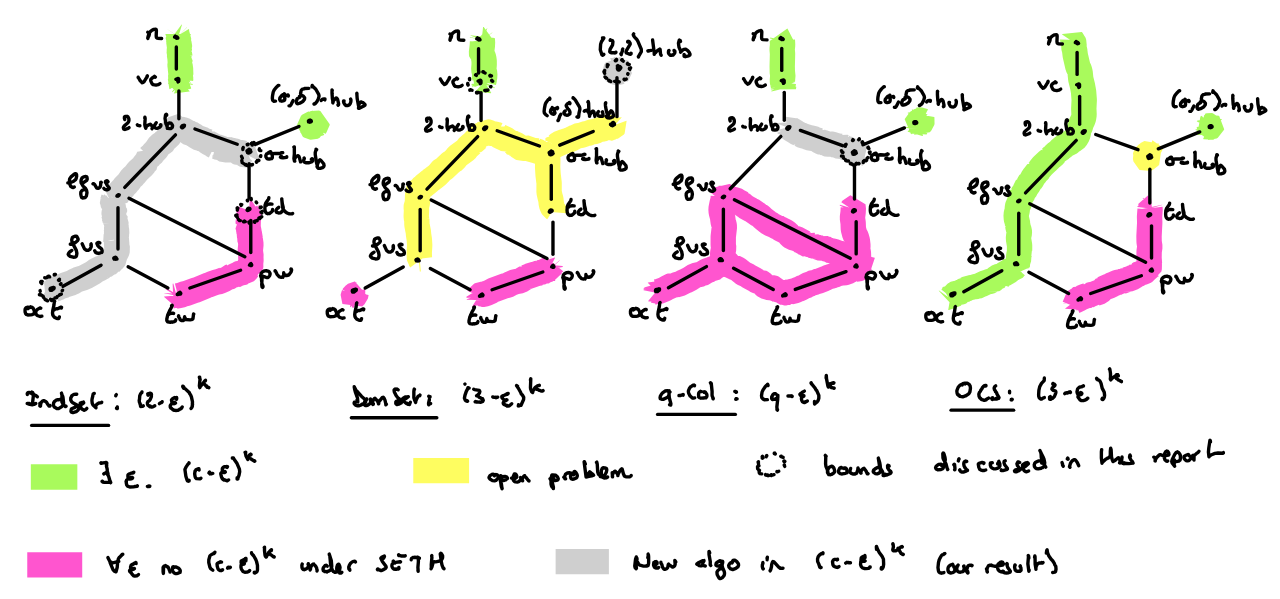
\includegraphics[width=\textwidth]{figures/state-of-the-art.png}
    \caption{Bounds for several \NP-hard problems. For each \NP-hard problem, we consider a constant $c$ and investigate whether there is an algorithm running in time $\O^\star((c-\varepsilon)^k)$ for some parameter $k$ and some $\varepsilon > 0$.}
    \label{fig:state-of-the-art}
\end{figure}

We now discuss the complexity of the four problems presented in the introduction of \refsec{section:preliminaries} (\prob{IndependentSet}, \prob{DominatingSet}, \prob{$q$-Coloring} and \prob{OddCycleTransversal}) through the prism of the hierarchy of parameters presented above. Everything described in this section is illustrated in \reffigure{fig:state-of-the-art}.

\medskip

First, note that \prob{VertexCover} and \prob{IndependentSet} are inherently the same problem. Finding an algorithm (or proving that no algorithm exists) for $\prob{VertexCover}/\pi$ for a parameter $\pi$ is equivalent to finding an algorithm (or proving that no algorithm exists) for $\prob{IndependentSet}/\pi$. This is because, for a graph $G$, the size of the maximum independent set and the size of the minimum vertex cover of $G$ sum to $n$, the number of vertices in $G$. Thus, answering the question "is there a \prob{VertexCover} of size $\leq k$?" can be rephrased as "is there no \prob{IndependentSet} of size $\geq n - k + 1$?".

\medskip

\reftheorem{theorem:treewidth-bound} already states the lower bounds parameterized by treewidth for all the problems discussed here. Actually, Loshktanov et al. proved that these lower bounds hold even when replacing treewidth by pathwidth \cite{lokshtanov2011known}.

In 2024, Esmer et al. introduces the notion of $\sdhub$ \cite{esmer2024fundamental}. In their paper, they wrote that $\sdhub$ reached "the arguably most restricted setting in which the lower bounds [of \cite{lokshtanov2011known}] hold". This statement was derived from the following theorems:

\begin{theorem}[\cite{esmer2024fundamental}]
    \label{theorem:sdhub-lowerbounds}
    For every $\varepsilon > 0$ there exist integers $\sigma, \delta \geq 1$ such that if there is an algorithm solving
    \begin{itemize}
        \item $\prob{IndependentSet}/\sdhub$ in time $\O^\star((2 - \varepsilon)^p)$, or
        \item $\prob{OddCycleTransversal}/\sdhub$ in time $\O^\star((3 - \varepsilon)^p)$, or
        \item $q\prob{-Coloring}/\sdhub$ in time $\O^\star((q - \varepsilon)^p)$,
    \end{itemize}
    given a $\sdhub$ of size at most $p$, then SETH fails.
\end{theorem}

\begin{theorem}[\cite{esmer2024fundamental}]
    \label{theorem:sdhub-upperbounds}
    For every $\sigma, \delta > 0$, 
    \begin{itemize}
        \item there exists $\varepsilon > 0$ such that every instance of $\prob{IndependentSet}/\sdhub$ can be solved in time $\O^\star((2 - \varepsilon)^p)$,
        \item there exists $\varepsilon > 0$ such that every instance of $\prob{OddCycleTransversal}/\sdhub$ can be solved in time $\O^\star((3 - \varepsilon)^p)$,
        \item there exists $\varepsilon > 0$ such that every instance of $q\prob{-Coloring}/\sdhub$ can be solved in time $\O^\star((q - \varepsilon)^p)$.
    \end{itemize}
    given a $\sdhub$ of size at most $p$.
\end{theorem}

While \reftheorem{theorem:sdhub-upperbounds} directly provides an algorithm for the three problems, \reftheorem{theorem:sdhub-lowerbounds} is not exactly cited as we want. Ideally, we would fix $\sigma$ and $\delta$ before $\varepsilon$ to establish a clear frontier in the hierarchy. But in the current citation, $\varepsilon$ is fixed before $\sigma$ and $\delta$. However, \reftheorem{theorem:sdhub-lowerbounds} gives us the following corollary:

\begin{corollary}
    \label{corollary:td-lowerbounds}
    For every $\varepsilon > 0$, if there is an algorithm solving
    \begin{itemize}
        \item $\prob{IndependentSet}/\td$ in time $\O^\star((2 - \varepsilon)^\td)$, or
        \item $\prob{OddCycleTransversal}/\td$ in time $\O^\star((3 - \varepsilon)^\td)$, or
        \item $q\prob{-Coloring}/\td$ in time $\O^\star((q - \varepsilon)^\td)$,
    \end{itemize}
    then SETH fails.
\end{corollary}

\begin{proof}
    Let us prove this for $\prob{IndependentSet}$; the proof for $\prob{OddCycleTransversal}$ and \prob{$q$-Coloring} is analogous.

    Suppose there exists an $\varepsilon$ such that there is an algorithm solving $\prob{IndependentSet}/\td$ in time $\O^\star((2 - \varepsilon)^\td)$. Take $\sigma$ and $\delta$ given for this $\varepsilon$ by \reftheorem{theorem:sdhub-lowerbounds}. Keep in mind that $\sigma$ and $\delta$ are constants (depending only on $\varepsilon$). Given a $\sdhub$ of size $p$, we can transform it into an elimination forest of depth $p + \sigma$ as described in the previous subsection (see \reffigure{fig:shub-to-treedepth}). By applying the algorithm for $\prob{IndependentSet}/\td$, we get a time complexity of $\O^\star((2 - \varepsilon)^{p + \sigma}) = \O^\star((2 - \varepsilon)^p)$. By \reftheorem{theorem:sdhub-lowerbounds}, SETH fails.
\end{proof}

Note that Esmer et al. did not establish the same bounds for $\prob{DominatingSet}/\sdhub$, leaving this as an open problem.

\medskip

Concerning bounds for other parameterizations of \prob{IndependentSet}, vertex cover is a well-studied parameter for this problem. An example of an algorithm for $\prob{VertexCover}/\vc$ (which directly gives an algorithm for $\prob{IndependentSet}/\vc$) is proposed in \cite[Theorem 3.2]{cygan2015parameterized} and runs in time $\O^\star(1.4656^\vc)$.

\medskip

As for \prob{DominatingSet}, it is already \NP-hard on bipartite graphs. Thus, we do not expect to find an algorithm for $\prob{DominatingSet}/\oct$  with running time $\O^\star((3-\varepsilon)^\oct)$ unless $\P = \NP$, which is a stronger conjecture than SETH. Moreover, an algorithm for $\prob{DominatingSet}/\vc$ can run in $\O^\star(2^\vc)$; we will discuss this in \refsec{section:domset-vc}. Other than that, the statues of $\prob{DominatingSet}/p$ for $\fvs$, $\td$, $\sdhub$ is still unknown.

\medskip

The work by Loshkatnov et al. \cite{lokshtanov2011known} was extended by Jaffke and Jansen, who proved a lower bound for $q\prob{-Coloring}/\lfvs$ \cite{jaffke2017fine}. They also proposed an algorithm running in time $\O^\star((q - 1.11)^\vc)$ for $q\prob{-Coloring}/\vc$.

\medskip

Finally, an algorithm for $\prob{OddCycleTransversal}/\oct$ was proposed by Loshkatnov et al. \cite{lokshtanov2012subexponential}, who developed an algorithm based on a branching guided by linear programming that runs in time $\O^\star(2.32^\oct)$. 

\subsubsection*{Our results}

The goal of this internship was to explore new upper and lower bounds under SETH. The main focus was initially on \prob{DominatingSet} and we studied parameters between $\oct$, $\tw$ and $\vc$. This proved to be an exceptionally challenging task, which had previously stymied researchers like Esmer et al. \cite{esmer2024fundamental}, who were unable to resolve $\prob{DominatingSet}/\sdhub$. However, we managed to give a proof for the special case of $\prob{DominatingSet}/\sdhub[2, 2]$ running in time $\O^\star(2^p)$, given a $\sdhub[2,2]$ of size $p$. While this algorithm addresses a special case, it effectively demonstrates our approach.  More details on this algorithm are discussed in \refsec{section:domset-22hub}.

\medskip

We then shifted our focus to a more approachable problem: \prob{IndependentSet}. In this area, we obtained results for $\prob{IndependentSet}/\oct$ and proposed an algorithm running in time $\O^\star(1.53^\oct)$ (see \refsec{section:indset-oct}). While the bound for $\prob{IndependentSet}/\td$ was already known by \refcorollary{corollary:td-lowerbounds}, we provided an alternative proof for this lower bound, which is presented in \refsec{section:indset-td}. Furthermore, we completed the hierarchy bounds for \prob{IndependentSet} by showing that for every $\sigma$, there exists an $\varepsilon$ such that $\prob{IndependentSet}/\shub$ can be solved in time $\O^\star((2- \varepsilon)^p)$, given a $\shub$ of size $p$. This algorithm is more complex and is not covered in this report. However, the proof has been documented for inclusion in a future paper.

\medskip

To further complete the hierarchy bounds for \prob{$q$-Coloring}, we extended the work of Esmer et al. by showing that for every $\sigma$, there exists an $\varepsilon$ for which there is an algorithm solving \prob{$q$-Coloring} in time $\O^\star((q-\varepsilon)^p)$, given a $\shub$ of size $p$. This algorithm is also not covered in this report, but the proof has been documented for future publication.